\documentclass[12pt, letterpaper]{report}% "letterpaper" matches US standard paper size.
\setcounter{tocdepth}{3}
% --- PACKAGES: Each one adds a capability to LaTeX ---
% Think of packages like Python imports or C #includes.


% ---------- Page Layout ----------
\usepackage[top=1in,bottom=1in,left=1in,right=1in]{geometry} % geometry lets you set margins. 1-inch all around is standard for reports.
% ---------- Encoding & Fonts ----------
\usepackage[utf8]{inputenc}% Allows special characters (é, ü, °) to be typed directly.
\usepackage[T1]{fontenc} % Ensures proper font encoding in the output PDF. Without this, copy-pasting from the PDF can produce garbled characters.
% ---------- Graphics & Figures ----------
\usepackage{graphicx}% THE core package for inserting images.
% Usage: \includegraphics[width=0.8\textwidth]{filename.png}
\graphicspath{{figuresSandiaAward/}}
\usepackage{float}% Gives you the [H] placement option for figures/tables. [H] means "put it HERE, not where LaTeX thinks is best." Very useful when you need a figure right after the text that references it.
\usepackage{subcaption}% Lets you put multiple images side-by-side in a single figure environment. Example: Figure 3(a) and Figure 3(b) next to each other.
% ---------- Tables ----------
\usepackage{booktabs} % Provides \toprule, \midrule, \bottomrule for professional-looking tables.
% Rule of thumb: NEVER use vertical lines in tables. Use booktabs rules instead.
\usepackage{tabularx}% Adds the tabularx environment, which lets columns auto-expand to fill width. Great for tables that need to span the full page width.
\usepackage{multirow}% Allows cells that span multiple rows in tables.
\usepackage{longtable}% For tables that are too long to fit on one page (like a Bill of Materials).
% ---------- Math ----------
\usepackage{amsmath}% The standard package for equations. Adds align, equation*, etc.
\usepackage{amssymb}% Extra math symbols (e.g., \therefore, \because, \pm).
\usepackage{siunitx}% Proper formatting for SI units.
\sisetup{per-mode=fraction}
\sisetup{exponent-product=\cdot}
% Usage: \SI{100}{\celsius}, \SI{10000}{psi}, \SI{10}{\centi\meter}
% This ensures consistent unit formatting throughout the document.
% ---------- Bibliography ----------
\usepackage[numbers, sort&compress]{natbib}
% IEEE-style numeric citations: [1], [2,3], [4-7]
% "sort&compress" turns [3,1,2] into [1-3]
% ---------- Cross-Referencing & Links ----------
\usepackage[
	colorlinks=true,
	linkcolor=blue,      % Internal links (sections, figures)
	citecolor=blue,      % Citation links
	urlcolor=blue         % URL links
]{hyperref}
% Makes all references, citations, and URLs clickable in the PDF.
% Set colorlinks=false if you want boxes instead of colored text.
% ---------- Captions ----------
\usepackage[
	font=small,           % Caption text slightly smaller than body
	labelfont=bf,         % "Figure 1:" is bold
	textfont=it            % The caption description is italic
]{caption}% Makes figure/table captions look more professional.
% ---------- Headers & Footers ----------
\usepackage{fancyhdr}% Customizable headers and footers.
\pagestyle{fancy}% Activate the fancy header/footer style.
\fancyhf{}% Clear all default header/footer content.
\fancyhead[L]{\small Team 019 --- Noble Aggie Labs}% Left header: team name.
\fancyhead[R]{\small Sandia Design Award}% Right header: course number.
\fancyfoot[C]{\thepage}% Center footer: page number.
\renewcommand{\headrulewidth}{0.4pt}% Thin line under the header. Set to 0pt to remove.
% ---------- Paragraph Formatting ----------
\usepackage{parskip}% Adds space between paragraphs instead of indenting the first line. This is more common in engineering reports than academic papers.
\setlength{\parindent}{0pt}% Explicitly remove paragraph indentation (parskip should handle this, but belt-and-suspenders doesn't hurt for readability).
% ---------- Line Spacing ----------
\usepackage{setspace}
\setstretch{1.15} % 1.5 line spacing for easy reading
%-------- For Box diagrams
\usepackage{tikz}
\usetikzlibrary{patterns}
\usetikzlibrary{patterns,intersections}
\usetikzlibrary{arrows.meta, positioning}
\usetikzlibrary{shapes.geometric}
% ---------- Appendix Support ----------
\usepackage[title,titletoc]{appendix} % Adds "Appendices" header and includes appendices in the Table of Contents. [title, titletoc] ensures they are labeled A, B, C
%----------- Title/Chapter formatting -----------------
\usepackage{titlesec}
% Format \chapter to look simple (no giant text, no separate page)
\usepackage{pdfpages}
% Allows you to insert entire PDF Pages (e.g., for Gantt charts, concept screening matrices) with \includepdf.
\usepackage{geometry}
%allows you to set margins and page size. 
\usepackage{mdframed}     % warning/note boxes
\usepackage{enumitem}     % list formatting
\usepackage{booktabs}     % tables
\usepackage{xcolor}       % color support
\usepackage{upgreek}
\usepackage{sectsty}

% Change the font size of all sections
\sectionfont{\large}

% Change the font size of all subsections
\subsectionfont{\normalsize}


\definecolor{warnred}{RGB}{180,30,30}
\definecolor{warnbg}{RGB}{255,235,235}
\definecolor{notebg}{RGB}{235,245,255}
\definecolor{noteblue}{RGB}{30,80,160}

\newmdenv[
  linecolor=warnred, backgroundcolor=warnbg,
  linewidth=1.5pt, innerleftmargin=10pt,
  innerrightmargin=10pt, innertopmargin=8pt,
  innerbottommargin=8pt, skipabove=10pt, skipbelow=6pt
]{warningbox}

\newmdenv[
  linecolor=noteblue, backgroundcolor=notebg,
  linewidth=1pt, innerleftmargin=10pt,
  innerrightmargin=10pt, innertopmargin=8pt,
  innerbottommargin=8pt, skipabove=10pt, skipbelow=6pt
]{notebox}


\titleformat{\chapter}
 {\LARGE\bfseries}  % format
 {}                % label
 {0em}                         % sep between label and title
 {}                            % before-code
\titlespacing*{\chapter}{0pt}{20pt}{10pt}  % left, before, after


\makeatletter
\g@addto@macro\appendix{%
 \titleformat{\chapter}[block]
	{\huge\bfseries\centering}
	{\appendixname\ \thechapter}
	{0em}
	{\vspace{0.5em}\\}%
}
\makeatother

% ---------- PDF Metadata ----------
\hypersetup{
	pdftitle={Sandia Design Award Report -- Passive Temperature Compensation Device},
	pdfauthor={Team 019: Noble Aggie Labs},
	pdfsubject={EME-185 Mechanical Systems Design Project, UC Davis},
}
%-----------For landscape pages----------
\usepackage{pdflscape}
\usepackage{pgfplots}
	\pgfplotsset{compat=1.18}
\usepackage{multirow}
\usepackage{array}      % for >{\raggedright\arraybackslash}
\usepackage{makecell}   % for \makecell
\usepackage{calc}
\usepackage{multicol}
\usepackage{mdframed}
\usepackage{wrapfig}

% In your preamble
\newcounter{mycounter}           % creates a counter, initialized to 0
\newcounter{sub}[mycounter]      % resets 'sub' when 'mycounter' increments
% ============================================================================
% SECTION 0.5: CUSTOM COMMANDS (Modular Helpers)
% ============================================================================
% These are reusable shortcuts. Define them once, use them everywhere.
% If a name or term changes, you only edit it in ONE place.


% --- Project-specific shortcuts ---
\newcommand{\projecttitle}{Passive Temperature Compensation Device}
\newcommand{\teamname}{Noble Aggie Labs}
\newcommand{\teamnumber}{019}
\newcommand{\sponsor}{Dr.\ Bradley Bon}
\newcommand{\organization}{Sandia National Laboratories}
\newcommand{\coursename}{EME 185}
\newcommand{\instructor}{Professor Jonathan Schofield}
\newcommand{\university}{University of California, Davis}
\newcommand{\ta}{Teaching Assistant Xiangpu Wang}
\newcommand{\duedate}{12 May 2026}
% --- Convenience commands for common terms ---
% Using these ensures consistent terminology throughout the report.
\newcommand{\device}{PTCD}
\newcommand{\degC}{^{\circ}\text{C}}    % Degree Celsius symbol, properly formatted
\newcommand{\requiredRelationship}{D_{\text{eff}} = A_1 (T_{\text{amb}} - T_{\text{ref}}) + A_0}
\newcommand{\transferFunction}{D_{\text{eff}}=\frac{dD_{\text{eff}}}{dX} \left[\frac{dL}{dT}\frac{dX}{dL}(T-T_{\text{ref}})+X\left(T_{\text{ref}} \right) \right]}

\newcommand{\Dcold}{D_{\text{eff}}(-60 \degC) = 383.5 \pm 19.2\ \mu m}
\newcommand{\Dhot}{D_{\text{eff}}(80 \degC) = 170.2 \pm 16.9\ \mu m}
\newcommand{\Dref}{D_{\text{eff}}(25 \degC) = 292.1 \pm 12.7\ \mu m}

\newcommand{\Thot}{\SI{80}{\degreeCelsius}} %Celcius
\newcommand{\Tcold}{\SI{-60}{\degreeCelsius}} %Celcius
\newcommand{\Tref}{\SI{25}{\degreeCelsius}} %Celcius
\newcommand{\specTempChange}{\SI{140}{\degreeCelsius}}

\newcommand{\specEAl}{\SI{69}{\giga \pascal}}
\newcommand{\specEALLV}{\SI{55}{\giga \pascal}}
\newcommand{\specEInv}{\SI{193}{\giga \pascal}}
\newcommand{\specEInc}{\SI{200}{\giga \pascal}}
\newcommand{\specActuatorCTE}{\SI{22.85}{\micro\meter\per\meter\per\celsius}} %Evaluated at 25C
\newcommand{\specMountCTE}{\SI{-30}{\micro\meter\per\meter\per\celsius}}
\newcommand{\specInvarCTE}{\SI{1.3}{\micro\meter\per\meter\per\celsius}}
\newcommand{\specInconelCTE}{\SI{13.2}{\micro\meter\per\meter\per\celsius}}
\newcommand{\specBellowsK}{\SI{3806}{\newton \per \meter}}
\newcommand{\specBellowsHeight}{\SI{22.86}{\milli \meter}} % = Neck 1 length + Neck 2 length + Conv free diameter = 2*(0.07") + 0.76"

\newcommand{\Xhot}{\SI{480.696}{\micro \meter}}
\newcommand{\Xcold}{\SI{213.289}{\micro \meter}}
\newcommand{\specLengthChange}{\SI{267.407}{\micro \meter}}
\newcommand{\govErrorProp}{u_x = \sqrt{\frac{\pi(\sigma_x^2+\sigma_y^2)}{2}}}
\newcommand{\govActuator}{\Delta L = L_0 \Delta T \alpha}
\newcommand{\govValve}{D_{\text{eff}} = \sqrt{\frac{2}{\pi}}}
\newcommand{\specPressure}{\SI{68.95}{\mega \pascal}}%  68.94757 MPa
\newcommand{\AoneExact}{\SI{-1.524e-3}{\frac{mm}{\degC}}}
\newcommand{\Aone}{\AoneExact \pm 5\%}
\newcommand{\AzeroExact}{\SI{0.254}{mm}}
\newcommand{\Azero}{\AzeroExact \pm 5\%}
\newcommand{\imageHeight}{4in} % Default image height for figures. Adjust as needed.
\newcommand{\specCrossSectArea}{\SI{6.3e-5}{\meter \squared}}
\newcommand{\specOrigActuatorLength}{\SI{32.991}{\milli \meter}}
\newcommand{\specMountEffLength}{\SI{37.991}{\milli\meter}} % Without washer thickness; = L_act + 5 mm gap

% Transfer function specifications

\newcommand{\GA}{\SI{1.216}{\frac{\micro \meter}{\celsius}}}
\newcommand{\GV}{\num{-1.253}}

% System Requirements
\newcommand{\ReqA}{The device shall passively restrict gas flow according to the Required Relationship $D = A_1 \Delta T + A_0$}
\newcommand{\ReqB}{The device should remain within a 10 cm $\times$ 10 cm $\times$ 10 cm mechanical envelope}
\newcommand{\ReqC}{The device shall operate under \specPressure\ internal pressure with Hydrogen gas, with thermal isolation of the actuator}

% Valve specifications
\newcommand{\SpecVA}{The valve subsystem shall passively control the effective orifice diameter as directly driven by the actuator at a conversion rate of $\frac{dD}{dL} = \GV$}
\newcommand{\SpecVB}{The valve subsystem shall not exceed a 10 cm $\times$ 5 cm $\times$ 10 cm mechanical envelope}
\newcommand{\SpecVCA}{The housing shall withstand an internal pressure of \specPressure}
\newcommand{\SpecVCB}{Wetted components shall maintain a hermetic seal at an internal pressure of \specPressure}
\newcommand{\SpecVCC}{Wetted components shall not permit Hydrogen diffusion or embrittlement}

% Actuator specifications
\newcommand{\SpecAA}{The actuator subsystem shall passively drive the valve subsystem in response to ambient temperature at a rate of $\frac{dL}{dT} = \GA$}
\newcommand{\SpecAB}{The actuator subsystem shall not exceed a 10 cm $\times$ 5 cm $\times$ 10 cm mechanical envelope}
\newcommand{\SpecACA}{The actuator shall remain thermally isolated from the gas flow \todo{Make this one more exact and out-come focussed.}}

% --- Tolerance values for specifications. --- 
% Fill in with real numbers as we find the relevant values 

%Valve tolerances
\newcommand{\dDdXTol}{$0.1\ \mu m$}
\newcommand{\dXdLTol}{$2.75\ \mu m$}
\newcommand{\pressureSF}{1.4}
\newcommand{\dXdTTol}{$0.01\ \mu m$}
\newcommand{\dLdTTolValve}{$0.1\ \mu m$}
\newcommand{\dTTol}{$1\ \degC$}
\newcommand{\FTolValve}{170 N}
\newcommand{\valveMEX}{100 mm}
\newcommand{\valveMEY}{5 mm}
\newcommand{\valveMEZ}{100 mm}

%Actuator tolerances
\newcommand{\dLdTTolAct}{$0.3\ \mu m$}
\newcommand{\FTolAct}{\FTolValve}

%Mount tolerances
\newcommand{\mountdLTol}{$12.5\ \mu m$}
\newcommand{\calRange}{$15\ \mu m$}
\newcommand{\calTol}{$5\ \mu m$}
\newcommand{\mountMEX}{100 mm}
\newcommand{\mountMEY}{130 mm}
\newcommand{\mountMEZ}{100 mm}

% --- Figure insertion helper ---
% This command simplifies inserting a figure with a caption and label.
% Usage: \insertfigure{width}{filename}{caption text}{fig:label}
%
% Parameters:
%   #1 = width relative to text width (e.g., 0.8 for 80%)
%   #2 = filename (without path if images are in the same directory)
%   #3 = caption text
%   #4 = label for cross-referencing (use fig:prefix by convention)
\newcommand{\insertfigure}[4]{%
	\begin{figure}[H]
		\centering
		\includegraphics[width=#1\textwidth]{#2}
		\caption{#3}
		\label{#4}
	\end{figure}
}

% --- TODO marker for draft mode ---
% Prints a bold red "TODO" so you can easily spot incomplete sections.
\usepackage{xcolor}
\usepackage{tocloft} % For listoftodos
% --- TODO marker ---
\newlistof{todos}{tod}{List of TODO's}
\newcommand{\todo}[1]{%
    \textbf{\textcolor{red}{[TODO: #1]}}%
    \addcontentsline{tod}{todos}{\protect\numberline{\thepage}#1}%
}


% ============================================================================
% BEGIN DOCUMENT
% ============================================================================


\begin{document}
\begin{titlepage}
    \thispagestyle{empty}   % No header/footer on the title page

    \begin{center}
        % --- Project Title & Report Type ---
        {\LARGE\bfseries \projecttitle}\\[8pt]
        {\large\bfseries SANDIA DESIGN AWARD REPORT}\\[32pt]

		\vspace{.5in}

        % --- Team Info ---
        {\large Prepared by the}\\[8pt]
        {\Large\bfseries \teamname}\\[12pt]
		{\Large\bfseries Team 019}\\[12pt]
        {Miguel Cuaycong, Jon Pizarro, Nicholas Metta,}\\
        {Isaiah Mathew, John Bodine, and Sam van der Veen}\\[32pt]

		\vspace{1in}

        % --- Course & Institution ---
        {\large EME 185: Mechanical Systems Design Project}\\
        {\large University of California, Davis}\\[24pt]
        
		\vspace{1in}

        % --- Advisors & Sponsors ---
        {Advised by \instructor\ and \ta}\\
        {Sponsored by {\sponsor}, {\organization}}
    \end{center}

    \vfill

    % --- Submission Deadline ---
    \begin{center}
        {\large\bfseries 12 MAY 2026}
    \end{center}

    \vspace{0.2in}

    % --- Copyright & Rights ---
    \begin{center}
        {\small
        \textcopyright\ 2026 by Miguel Cuaycong, Jon Pizarro, Nicholas Metta,\\
        Isaiah Mathew, John Bodine, and Sam van der Veen\\[8pt]
        \textit{All rights reserved. No part of this report may be reproduced}\\
        \textit{without consent from the authors, UC Davis,}\\
        \textit{or Sandia National Laboratories.}
        }
    \end{center}
\end{titlepage}


\newpage  % Start the body of the report on a fresh page
\section*{Problem Statement}

	Sandia National Laboratories conducts numerous experiments requiring the flow of precisely controlled Hydrogen gas.
	These experiments are sensitive to fluctuations in temperature; the flow must be adjusted to compensate for these changes.
	However, power and space constraints prohibit the use of embedded control systems.
	Sandia commissioned the Noble Aggie Labs from UC Davis to design and prototype a Passive Temperature Compensation Device (\device)
	that controls high-pressure Hydrogen gas flow and thermomechanically adjusts its effective orifice diameter according to the relationship
    $D_{\text{eff}} = A_1 (T_{\text{amb}} - \SI{25}{\celsius}) + A_0$,
    where $A_1 = \Aone$, $A_0 = \Azero$, and $(\SI{-60}{\celsius} \leq T_{amb} \leq \SI{80}{\celsius})$\cite{ref_sandiaprompt}.
    The \device\ must contain, seal, and restrict the gas at a maximum pressure of \specPressure, resist Hydrogen diffusion and embrittlement, and fit within a $(\SI{10}{\centi\meter})^3$ mechanical envelope.
    
\section*{Sandia Impact}

Sandia National Laboratories develops technologies that support national security and advance scientific discovery, often under extreme environmental constraints 
where active control systems are impractical. The \device\ directly addresses this problem: precision flow control of high-pressure hydrogen gas achieved entirely through 
geometry and material selection, with no power source or control logic required. This approach aligns with the National Academy of Engineering Grand Challenge of engineering the tools of scientific 
discovery, as the device enables experiments requiring precisely controlled gas flow under conditions where embedded electronics are prohibited. Beyond Sandia's laboratories, 
passive temperature-compensating devices have broad applicability in aerospace, precision research, and high-pressure industrial systems, demonstrating that sub-millimeter precision 
flow control is achievable through purely mechanical means.

    \section*{Design Approach}

The primary design requirement is that orifice flow area vary linearly with ambient temperature over the specified temperature range. The system was divided into 
two subsystems: the actuator, which thermomechanically responds to ambient temperature, and the valve, which restricts gas flow as driven by the actuator. For the 
combined system to produce a first-order linear output, each subsystem must independently exhibit a single degree of freedom and a linear response. Candidate designs 
for each subsystem were evaluated against defined criteria using a scoring matrix, which prioritizes linearity and simplicity.

For the actuator, candidates included a bimetallic coil, wax bladder, and piston-cylinder assembly and were evaluated against a thermal expansion rod. 
All the other candidates were rejected on the basis of nonlinearity or mechanical complexity. Aluminum was selected for the rod material due to its high, consistent
coefficient of thermal expansion (CTE) and machinability. Allvar 30 was selected for the mount instead of steel because its negative CTE increases rather than reduces actuator displacement.

For the valve, all conventional valve types were evaluated, including stopper, panel, rotary, and pinch valve configurations, and were rejected for their 
inability to produce a linear flow area response. A novel geometry was developed in which two plates with square orifices are rotationally offset by 45 degrees. 
The overlapping area between the orifices varies linearly with relative plate displacement, satisfying the linearity requirement through geometry alone, with a single moving component.

\section*{Final Solution}

    The final design of the Passive Temperature Compensation Device, pictured in Figure \ref{fig:assembly_combined}, successfully meets the above specifications, thermomechanically controlling Hydrogen gas flow with extreme precision
    using a simple, compact architecture.

  \begin{figure}[h]
    \centering
    \begin{subfigure}[b]{0.48\textwidth}
        \centering
        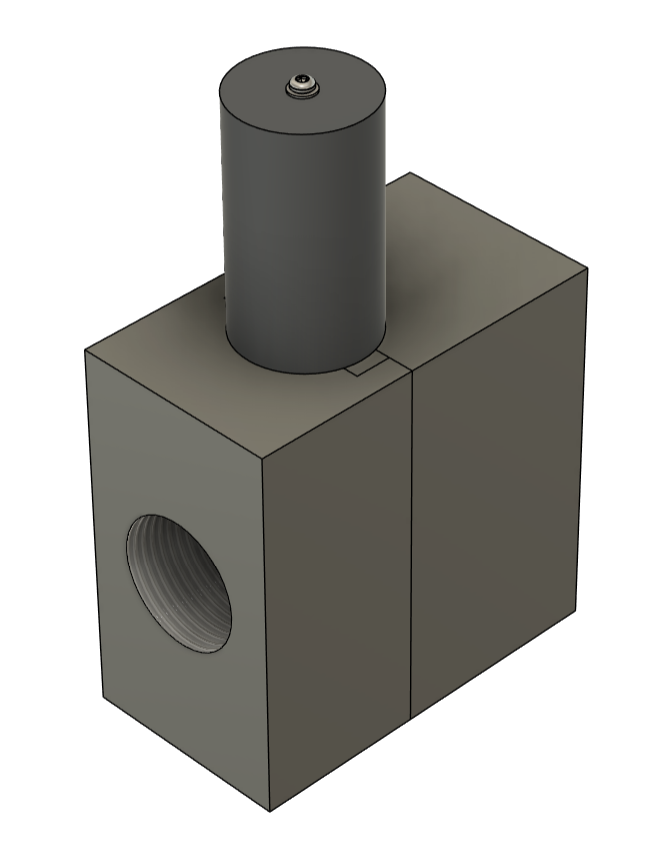
\includegraphics[height=0.35\textheight, keepaspectratio]{full_assembly.png}
        \caption{Complete assembly}
        \label{fig:mainIsometric}
    \end{subfigure}
    \hfill
    \begin{subfigure}[b]{0.48\textwidth}
        \centering
        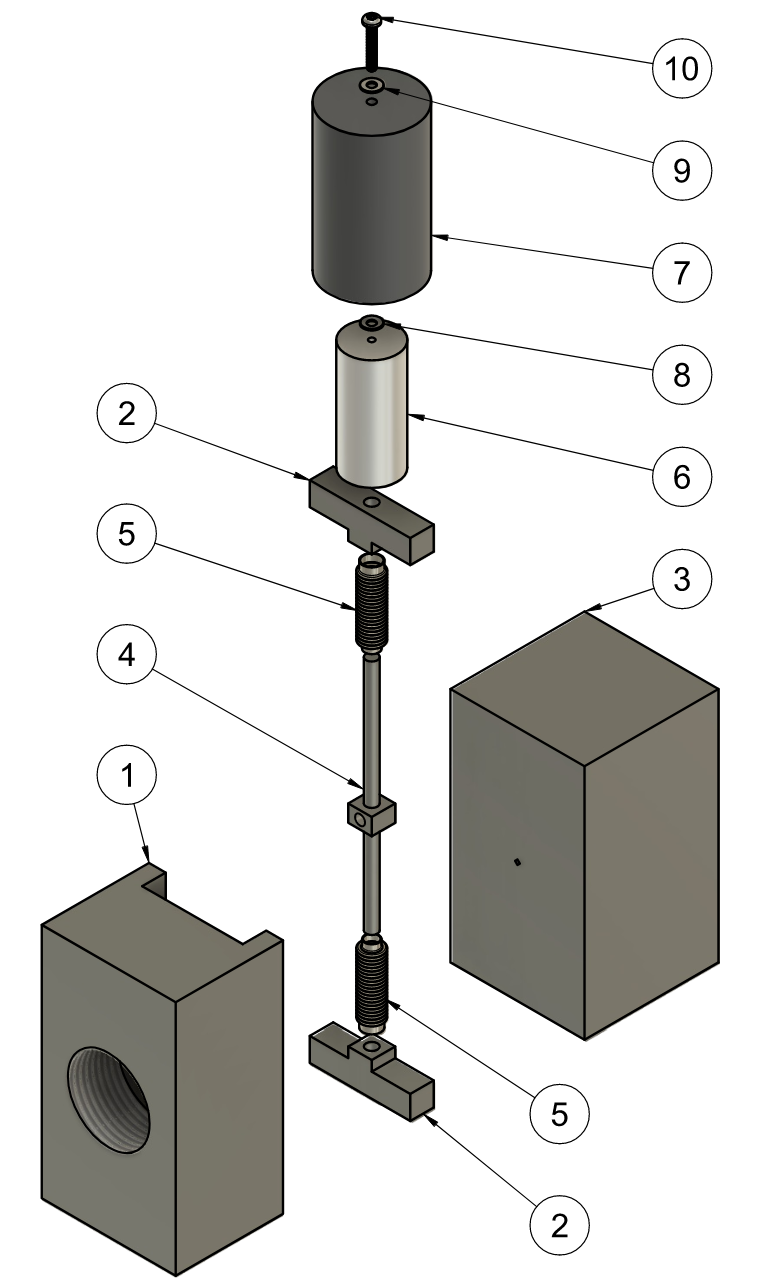
\includegraphics[height=0.40\textheight, keepaspectratio]{exploded_callout.png}
        \caption{Complete assembly exploded view}
        \label{fig:mainExploded}
    \end{subfigure}
    \caption{Overall \device\ assembly and exploded view highlighting internal components.}
    \label{fig:assembly_combined}
\end{figure}

    The bimetallic actuator, the functional core of the \device, leverages the difference in Coefficients of Thermal Expansion between two metals. An Aluminum 6061 expansion rod (6) nests inside a hollow, cylindrical ALLVAR mount (7).
    Aluminum's expansion rate $\alpha_{\text{Al}} \approx \specActuatorCTE$\cite{ref_NASA_specs_Al}; it expands when heated. ALLVAR, a proprietary technology made by ALLVAR Alloys, shrinks when heated at a rate of $\alpha_{\text{ALLV}} \approx \specMountCTE$ \cite{ref_AllvarAlloys}.
    The mount, secured at its base, lowers the assembly as it shrinks while the aluminum rod, fastened to the mount from above by the screw-washer assembly (8, 9, 10), simultaneously expands downwards.
    Temperature decrease produces the reverse effect.
    The assembly linearly translates the ambient temperature into compound relative displacement according to the governing equation $\Delta L = \left( L_{\text{actuator}} \alpha_{\text{Al}} - L_{\text{mount}} \alpha_{\text{ALLV}} \right) \Delta T$.
    At full range, the actuator drives the valve \SI{267}{\micro\meter}.

    \begin{wrapfigure}{l}{.3\textwidth}
        \centering
        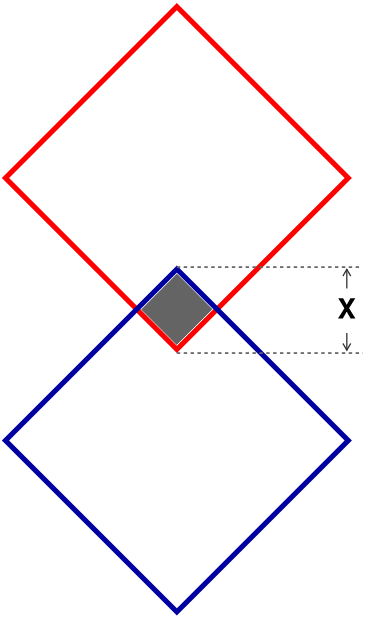
\includegraphics[height=2in]{orifice.png}
        \caption{Orifice geometry}
        \label{fig:orifice}
    \end{wrapfigure}

    The valve subsystem comprises the central orifice, structural housing, and associated hermetic seals. A novel orifice architecture was required to achieve the linear relationship between displacement (provided by the actuator) and effective diameter.
    While most gas flow control valves exhibit a first-order change in orifice area, the specified temperature-diameter translation required that the orifice remain a regular polygon.
    The \device\ achieves this with a unique diamond-overlap approach, pictured in Figure \ref{fig:orifice}.
    The valve stem (4) and housing outlet (3) each contain a small square hole rotated \SI{45}{\degree}. When assembled, these are pressed against one another and slightly offset such that gas may only flow through the overlap between them.
    As the actuator drives the valve stem downwards, its diamond (pictured as blue in Fig. \ref{fig:orifice}) descends relative to the fixed diamond on the housing, shrinking the overlap and restricting the flow.
    Their \SI{45}{\degree} rotation allows the orifice to remain a square, resulting in a linear output.
    As calculated in Appendix~\ref{app:der:TF}, the bimetallic actuator and diamond orifice combine to produce the exact linear relationship required by Sandia.
    
    The orifice is cut using wire electrical-discharge machining, allowing 
    for a very small minimum corner radius (0.076 mm), which is critical for achieving the required precision in flow control. All contact surfaces are coated with a physical vapor deposition (PVD) coating to prevent galling.

    The valve housing components are responsible for maintaining the structural integrity of the device under the specified internal pressure of \SI{68.95}{\mega\pascal}.
    Pressure-stress calculations in Appendix \ref{app:der:P} verify that the housing can withstand this internal pressure.
    The housing includes the valve inlet (1), which connects to the gas source, the housing center pieces (2), which contain the valve internal components, and the valve outlet (3), which directs the flow through the orifice.
    The housing is designed with a compact form factor to meet the specified mechanical envelope while providing sufficient material thickness and support to withstand the internal pressure without deformation that could affect the orifice geometry.
    The housing is fabricated from Invar 36, a one-of-a-kind alloy renowned in the aerospace industry for its low CTE $(\alpha \approx \SI{1.3}{\micro\meter\per\meter\per\celsius})$ \cite{ref_Carpenter_Inv, ref_Invar_1897, ref_Invar_1920},
    ensuring that unwanted thermal expansion is minimized.

    Sealing of the valve is achieved through a combination of welded joints and two Inconel 718 bellows (5) \cite{ref_miniflex_design}. The bellows provide a hermetic seal while allowing for the 
    necessary axial motion of the valve stem, ensuring that the device can operate under the specified internal pressure without leakage. 
    The use of two bellows (upper and lower) provides a balanced response to the internal pressure, minimizing the net force on the valve stem and thus reducing the 
    load on the actuator. This design choice is critical for maintaining the precision of the device, as it prevents deformation of the valve components under pressure 
    that could otherwise affect the orifice geometry.

    Weld joints are used throughout the assembly to enable simple mates with minimal degrees of freedom, contributing to the overall robustness
    of the design \cite{ref_steen2010laser}. Electron beam welding was selected for its ability to create strong, precise welds, all of which will be verified through full radiographic inspection.

    Calibration of the device is performed during final assembly through the use of a manually torqued adjustment screw and a Belleville washer (8). By adjusting 
    the preload on the Belleville washer via the adjustment screw and consequently the vertical position of the valve orifice, the user can ensure that the actuator's 
    motion corresponds to the required orifice diameter at the reference temperature of \SI{25}{\degreeCelsius}.
    This eliminates any constant-offset error introduced by stochastic machining and assembly errors.

    Throughout the design, exact interface dimensions and tolerances were carefully calculated to ensure that components fit together with the necessary precision to meet the required specifications. 
    The design also incorporates features to facilitate assembly and encourage access for welding. Compared to previous iterations, the final design achieves a more compact and robust configuration with fewer unique parts.


\section*{Evaluation and Verification}

    After completion of the final design iteration, verification of the \device\ control output was conducted both analytically and numerically.
    Analytical verification consisted of derivation and calculation of the passive system control transfer function, commonly used in the field of control systems \cite{ref_Nise}.
    The resulting computation, represented graphically in Appendix~\ref{app:modeling}, analytically estimated the effect of machining errors, thermal expansion of every part, and spring reactions from the bellows.
    The transfer function produced the system output results shown in Figure \ref{fig:TF_plot}, verifying satisfaction of the required relationship despite these sources of error.
    The gold line, the function-estimated output, fits well within the tolerated error band, demonstrating a real prototype would likely produce similarly satisfactory results.

    \insertfigure{0.9}{TF_plot.png}{System Verification}{fig:TF_plot}

    Numerical verification of the \device\ will consist of a computational prototype to test against various failure modes.
    This is still in-progress and will be completed by the end of the academic quarter. The following section discusses this verification in more detail.

\section*{Improvements and Future Work}

    The current \device\ design reliably accomplishes the specified requirements under extreme temperature and pressure conditions. Further computational verification is currently in progress, including finite-element stress analysis, dynamic fluid pressure analysis, and thermal analysis to further validate the design prior to physical testing. The primary challenge anticipated in future development is manufacturing repeatability, which should be the focus of subsequent design iterations.

    The client, after fabricating the first prototype, will physically validate the design with two tests: a dry test, in which the device is subjected to a controlled ambient temperature and the effective orifice diameter is optically measured; and a wet test, in which fluid flows at a specified inlet pressure and ambient temperature for 60 seconds while pressure drop is recorded.

\begin{thebibliography}{99}

    \bibitem{ref_sandiaprompt}
    B.\ Bon, ``Passive Temperature Compensation Device --- Project Prompt,''
    Sandia National Laboratories, SAND2025-15446O, 2025.

    \bibitem{ref_NASA_specs_Al}
    R.\ F.\ Muraca and J.\ S.\ Whittick, \textit{Materials Data Handbook:
    Aluminum Alloy 6061}, 2nd ed., Western Applied Research \& Development,
    Inc., NASA CR-123772, May 1972. Available:
    \url{https://ntrs.nasa.gov/api/citations/19720022808/downloads/19720022808.pdf}
    [Accessed: May 8, 2026].

    \bibitem{ref_AllvarAlloys}
    ALLVAR Alloys, \textit{What is Negative Thermal Expansion?}, ALLVAR Alloys,
    2026. [Online]. Available:
    \url{https://allvaralloys.com/negative-coefficient-of-thermal-expansion-products-applications/round-bar-and-tube/}
    [Accessed: May 8, 2026].

    \bibitem{ref_Carpenter_Inv}
    Carpenter Technology Corporation, \textit{Invar 36 Datasheet}, Carpenter
    Technology Corporation, 2025. [Online]. Available:
    \url{https://www.carpentertechnology.com/hubfs/7407324/Material%20Saftey%20Data%20Sheets/Invar%2036.pdf}
    [Accessed: May 8, 2026].

    \bibitem{ref_Invar_1897}
    C.-\'{E}.\ Guillaume, ``Recherches sur les aciers au nickel. Dilatations
    aux temp\'{e}ratures \'{e}lev\'{e}es; r\'{e}sistance \'{e}lectrique,''
    \textit{Comptes Rendus de l'Acad\'{e}mie des Sciences}, vol.~125,
    pp.~235--238, 1897. Available:
    \url{https://gallica.bnf.fr/ark:/12148/bpt6k3080s/f239.item}
    [Accessed: May 8, 2026].

    \bibitem{ref_Invar_1920}
    C.-\'{E}.\ Guillaume, ``Invar and Elinvar,'' Nobel Lecture, Nobel Prize
    in Physics, Stockholm, Sweden, Dec.\ 11, 1920. Available:
    \url{https://www.nobelprize.org/prizes/physics/1920/guillaume/lecture/}
    [Accessed: May 8, 2026].

    \bibitem{ref_miniflex_design}
    Mini-Flex Corporation, \textit{Metal Bellows Design Guide}, Mini-Flex
    Corporation, Watervliet, NY. [Online]. Available:
    \url{https://mini-flex.com/metal-bellows-design-guide/}
    [Accessed: Feb. 23, 2026].

    \bibitem{ref_steen2010laser}
    W.~M. Steen and J.~Mazumder, \textit{Laser Material Processing}, 4th ed.,
    Springer, London, UK, 2010.

    \bibitem{ref_Nise}
    N.~S. Nise, \textit{Control Systems Engineering}, 8th ed.\ Hoboken, NJ:
    Wiley, 2019.

    \bibitem{ref_shigley}
    J.~E. Shigley, C.~R. Mischke, and R.~G. Budynas,
    \textit{Mechanical Engineering Design}, 8th~ed., McGraw-Hill, New York,
    2006, Eq.~8-27, Table~8-15.

\end{thebibliography}

\newpage
\begin{appendices}
\appendix

\titleformat{\chapter}[block]
  {\Large\bfseries}
  {\appendixname\ \thechapter\ -\ }
  {0pt}
  {}
\titlespacing*{\chapter}{0pt}{6pt}{10pt}


\chapter{Derivations and Calculations}
\label{app:derivations}

% ------------------------------------------------------------
\section{System Output of the \device}
\label{app:der:TF}
% ------------------------------------------------------------

The Required Relationship given in the problem statement

$$\requiredRelationship$$

where

$$A_1 = \Aone$$
$$A_0 = \Azero$$
$$T_{\text{ref}} = \SI{25}{\celsius}$$
$$(\SI{-60}{\celsius} \leq T_{amb} \leq \SI{80}{\celsius})$$

stipulates a linear temperature-diameter control output with the following endpoints:

$$\Dcold$$
$$\Dhot$$

The \device\ is tuned to produce exactly these results. Each subsystem contributes one control derivative to the system output relation

\begin{equation}
    D_{\device} = \frac{dL}{dT} \frac{dX}{dL} \frac{dD}{dX} \Delta T + D(T_{\text{ref}})
\end{equation}

$\frac{dL}{dT}$ is driven by the actuator subsystem, which converts changes in temperature to length change according to the relation

\begin{equation}
    \begin{aligned}
        \frac{dL}{dT} &= \left( L_{\text{core}} \alpha_{\text{Al}} - L_{\text{mount}} \alpha_{\text{ALLV}} \right) \\
        &= \left[ \left( \specOrigActuatorLength \right) \left( \specActuatorCTE \right) - \left( \specMountEffLength \right) \left( \specMountCTE \right) \right] \\
        &= \SI{1.91}{\micro\meter\per\celsius}
    \end{aligned}
\end{equation}

As the actuator expands and $L$ increases, it directly drives the valve stem. The orifice height $X$, defined in Figure \ref{fig:orifice}, decreases as much as $L$ increases.
Thus, $\frac{dX}{dL} = -1$.

$\frac{dD}{dX}$ is driven by the valve subsystem orifice geometry.
The area of the orifice is defined by its side length
$$A = s^2$$
The effective diameter, $D_\text{eff}$, is the diameter of a circle of equal area,
$A = \frac{\pi}{4} D_\text{eff}^2$.
The \device\ orifice is the diamond-shaped overlap between two $45^\circ$-rotated squares with area $A = s^2$, where $s$ is the side length of the overlap diamond.
Since the actuator drives the orifice height $X$,
the Pythagorean theorem gives $s = X/\sqrt{2}$, so:
\begin{equation}
    \frac{\pi}{4} D_\text{eff}^2 = \frac{X^2}{2}
    \qquad \Longrightarrow \qquad
    D_\text{eff} = \sqrt{\frac{2}{\pi}}\, X
    \label{eq:app_Deff_X}
\end{equation}
Thus,
\begin{equation}
    \frac{dD}{dX} = \sqrt{\frac{2}{\pi}} = 0.798
\end{equation}

Finally, the reference orifice diameter is set by the position of the valve stem hole such that
\begin{equation}
    D_{ref} = \SI{0.254}{\milli\meter}
\end{equation}

therefore
\begin{equation}
    D_{\device} = (\SI{1.91}{\micro\meter\per\celsius})(-1)(0.798) \Delta T + \SI{0.254}{\milli\meter}
\end{equation}
as prescribed.

\newpage
% ------------------------------------------------------------
\section{Pressure Vessel Structural Verification}
\label{app:der:P}
% ------------------------------------------------------------

The valve housing is modelled as a thick-walled cylinder of Invar~36
under internal pressure $P = 68.95$~MPa. Principal stresses\cite[Sec.~3-14]{ref_shigley} at the
\emph{inner wall} (worst case) are:
\begin{align}
    \sigma_\theta
        &= P\left(\frac{r_o^2+r_i^2}{r_o^2-r_i^2}\right)
         = 68.95\left(\frac{19.53^2+9.53^2}{19.53^2-9.53^2}\right)
         \approx 112.1\ \text{MPa}
    \quad\text{(hoop)} \\
    \sigma_r   &= -P \approx -68.95\ \text{MPa}
    \quad\text{(radial)} \\
    \sigma_z
        &= P\left(\frac{r_i^2}{r_o^2-r_i^2}\right)
         \approx 21.6\ \text{MPa}
    \quad\text{(longitudinal)}
\end{align}
The von~Mises equivalent stress is:
\begin{equation}
    \sigma_\text{vm}
    = \sqrt{\frac{(\sigma_\theta-\sigma_r)^2
                 +(\sigma_r-\sigma_z)^2
                 +(\sigma_z-\sigma_\theta)^2}{2}}
    \approx 156.8\ \text{MPa}
\end{equation}
With a material yield strength $S_y = 370$~MPa (Invar~36):
\begin{equation}
    FS = \frac{S_y}{\sigma_\text{vm}}
               = \frac{370}{156.8}
               \approx 2.36
\end{equation}
For weldments, the ASME~B31.3 minimum wall thickness (with $E = 1.0$ from 100\%
radiographic inspection) is:
\begin{equation}
    t_\text{min}
    = \frac{P\,D_o}{2(S\,E\,W + P\,Y)}
    = \frac{68.95 \times 39.06}{2(246.7 + 27.6)}
    \approx 5.17\ \text{mm}
    \;<\;
    t_\text{actual}
\end{equation}
Both checks confirm structural viability with comfortable margins.

\chapter{Computational Modeling: System Transfer Function}
\label{app:modeling}

    Figure \ref{fig:TF} represents the transfer function, derived and encoded into C++ to verify the expected results from the \device.
    The details of its derivation are too in-depth for presentation here, but the curious reader might find the following summary enlightening.

    Each block represents a subpart of the system, which takes one value as its input and outputs a new value.
    The ambient temperature is input into each of eight independent parts. The first row of blocks represents temperature adjustment as each part equilibrates with the hotter internal gas.
    The second row represents the thermal expansion of every part, including those which are not supposed to expand.
    The resulting length values of these mechanically coupled parts are entered into a spring-force balance (a system of eight linearly independent equations), giving the final length of each part.
    These are properly summed to find the position of each orifice, whose difference comprises the height of the final overlap between them.
    This is then converted to the effective diameter.

    \insertfigure{0.9}{TF.png}{Transfer Function Block Diagram.}{fig:TF}

\chapter{Bill of Materials and Assembly Drawings}
\label{app:drawings}

\includepdf[pages=1, fitpaper=true, landscape=true]{BOM.pdf}
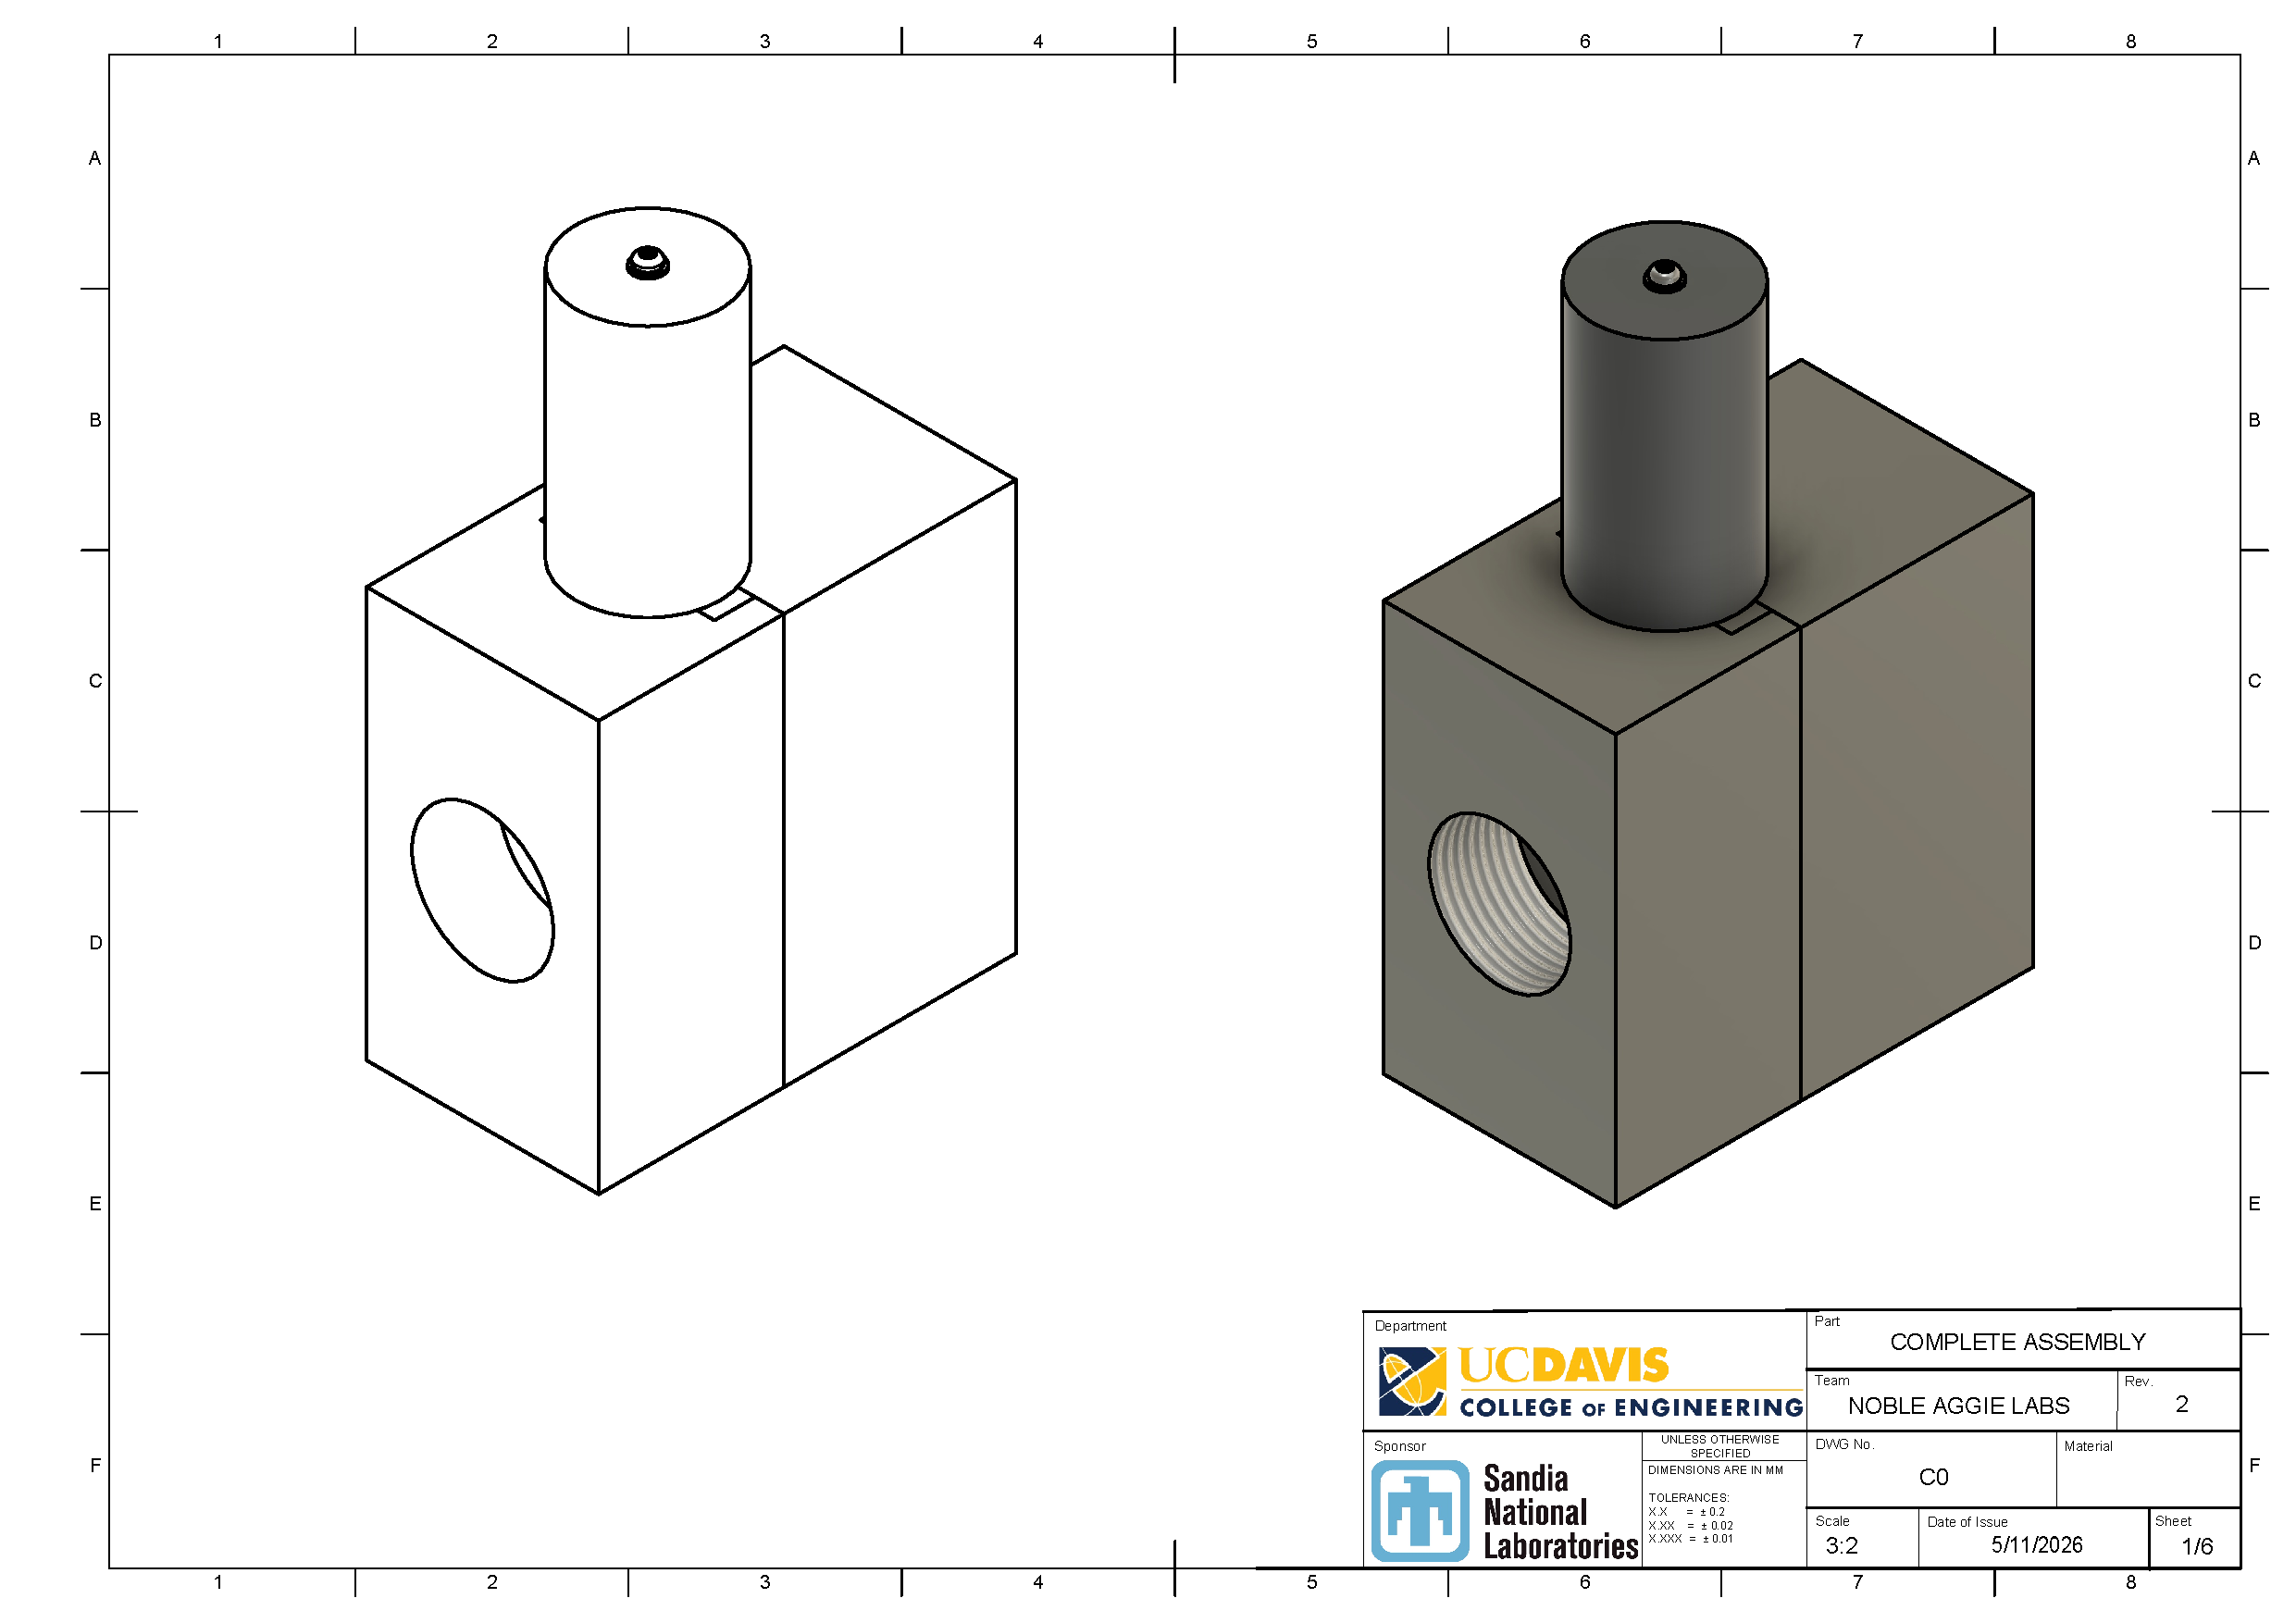
\includepdf[pages=1-6, fitpaper=true, landscape=true]{AssemblyDrawings.pdf}

\end{appendices}
\end{document}